% Chapter 1

\chapter{Data Preprocessing} % Main chapter title

\label{Chapter2} % For referencing the chapter elsewhere, use \ref{Chapter1} 

\lhead{\emph{Data Preprocessing}} % This is for the header on each page - perhaps a shortened title

%----------------------------------------------------------------------------------------

\section{Data Cleaning}

 I made use of relevant function in Pandas to check for missing values, duplicates, and outliers. However, the data was quite clean already, and barely required any initial cleaning. The table below shows no null values in any of the columns:

\begin{table}[htbp]
    \centering
    \rowcolors{1}{orange!20}{white}
    \begin{tabular}{|>{\columncolor{orange!50}}c|c|}
        \hline
        \rowcolor{orange!50}
        \textbf{Column Name} & \textbf{Total Null Values} \\
        \hline
        Invoice ID & 0 \\
        Branch & 0 \\
        City & 0 \\
        Customer type & 0 \\
        Gender & 0 \\
        Product line & 0 \\
        Unit price & 0 \\
        Quantity & 0 \\
        Tax 5\% & 0 \\
        Total & 0 \\
        Date & 0 \\
        Time & 0 \\
        Payment & 0 \\
        COGS & 0 \\
        Gross margin percentage & 0 \\
        Gross Income & 0 \\
        Rating & 0 \\
        \hline
    \end{tabular}
    \caption{There were no duplicates or outliers}
    \label{tab:alternating_colors}
\end{table}

% If you are writing a thesis (or will be in the future) and its subject is technical or mathematical (though it doesn't have to be), then creating it in \LaTeX{} is highly recommended as a way to make sure you can just get down to the essential writing without having to worry over formatting or wasting time arguing with your word processor.

% \LaTeX{} is easily able to professionally typeset documents that run to hundreds or thousands of pages long. With simple mark-up commands, it automatically sets out the table of contents, margins, page headers and footers and keeps the formatting consistent and beautiful. One of its main strengths is the way it can easily typeset mathematics, even \emph{heavy} mathematics. Even if those equations are the most horribly twisted and most difficult mathematical problems that can only be solved on a super-computer, you can at least count on \LaTeX{} to make them look stunning.

%----------------------------------------------------------------------------------------

\section{DateTime}

The main task here was to make use of the existing Date and Time features and extract utilizable features. Other than this, I dropped a few irrelevant columns in the preprocessing phase. After doing so, I was able to get the following new features:


\begin{table}[htbp]
    \begin{minipage}{0.45\linewidth}
        \centering
        \rowcolors{1}{green!20}{white}
        \begin{tabular}{|>{\columncolor{green!50}}c|c|}
            \hline
            \rowcolor{green!50}
            \textbf{Date} & \cellcolor{green!50}\textbf{Time} \\
            \hline
            1/5/2019 & 13:08 \\
            3/8/2019 & 10:29 \\
            3/3/2019 & 13:23 \\
            1/27/2019 & 20:33 \\
            2/8/2019 & 10:37 \\
            \hline
        \end{tabular}
        \caption{Original Features}
        \label{tab:alternating_colors}
    \end{minipage}
    \hfill
    \begin{minipage}{0.45\linewidth}
        \centering
        \rowcolors{1}{green!20}{white}
        \begin{tabular}{|>{\columncolor{green!50}}c|c|c|}
            \hline
            \rowcolor{green!50}
            \textbf{Date} & \cellcolor{green!50}\textbf{Time} & \cellcolor{green!50}\textbf{Duration} \\
            \hline
            1 & 3 & 13 \\
            3 & 8 & 10 \\
            3 & 3 & 13 \\
            1 & 27 & 20\\
            2 & 8 & 10 \\
            \hline
        \end{tabular}
        \caption{New Features}
        \label{tab:extended_features}
    \end{minipage}
\end{table}



%----------------------------------------------------------------------------------------

\section{Encoding}

The main task here was to make use of the existing Date and Time features and extract utilizable features. Other than this, I dropped a few irrelevant columns in the preprocessing phase. After doing so, I was able to get the following new features:

\vspace{2cm}

\begin{table}[htbp]
    \centering
    \rowcolors{1}{orange!20}{white}
    \begin{tabular}{|>{\columncolor{orange!50}}c|c|}
        \hline
        \rowcolor{orange!50}
        \textbf{Column Name} & \textbf{Total Null Values} \\
        \hline
        Branch & 3 \\
        City & 3 \\
        Customer type & 2 \\
        Gender & 2 \\
        Product line & 6 \\
        Unit price & 943 \\
        Quantity & 10 \\
        Tax 5\% & 990 \\
        Total & 990 \\
        Payment & 3 \\
        COGS & 990 \\
        Gross margin percentage & 1 \\
        Gross Income & 990 \\
        Rating & 61 \\
        \hline
    \end{tabular}
    % \caption{there were no duplicates or outliers}
    \label{tab:alternating_colors}
\end{table}



\begin{figure}[h]
    \centering
    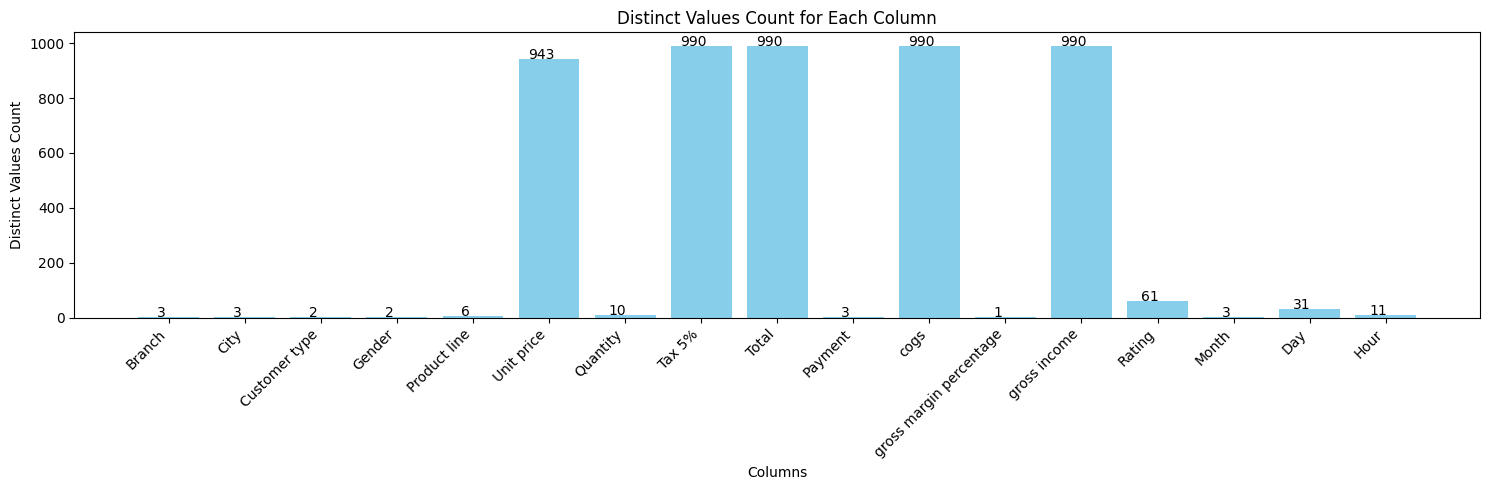
\includegraphics[width=1\textwidth]{Chapters/ch2/testing .png}
    % \caption{This is an example image.}
    % \label{fig:example}
\end{figure}
% \subsection{About this Template}

\newpage 
From this we can identify the feature ‘gross margin percentage’ is not of any use, since it has only 1 distinct value. Which means it cannot have any correlation with other features, hence, it will not hold any importance in the variation of any target variable that we may choose when training a model.

\begin{table}[htbp]
    \centering
    \resizebox{\textwidth}{!} & \textbf{Total} & \textbf{Unit price} & \textbf{COGS} & \textbf{Gross income} \\
        \hline
        \textbf{Total} & 0.002515 & 0.00277 & 0.022301 & 0.70551 & 0.036442 & 1.0 & 1.0 & 0.633962 & 1.0 & 1.0 \\
        \hline
        
    \end{tabular}%
    }
    % \caption{Scaled Table with Headers, Larger Font, and Wider Rows}
    \label{tab:scaled_table}
\end{table}



\subsection{Label Encoding}

suitable for ordinal variables, where there is an inherent order or ranking among the categories. For example, in our dataset, the days are ordinal because they have a clear and meaningful sequence. Each day follows the previous one in a systematic and sequential manner. Label encoding assigns integers based on this order, with the assumption that there is a linear relationship between the categories. This simplifies the representation of this variable while preserving the ordinal information. Hence, I’m using Label Encoding for the columns ‘Day’, ‘Month’ and ‘Hour.

\subsection{One Hot Encoding}

suitable for nominal variables, where there is no inherent order among the categories. Nominal variables represent categories with no implied order or ranking. In our dataset, columns like 'Branch', 'City', 'Gender', 'Product line', ‘Customer type’, and 'Payment' fall into this category.
\newline

The decision to use one-hot encoding is influenced by the understanding that these variables represent categories without any natural order. One-hot encoding creates binary columns for each category, providing a binary indicator (0 or 1) for the presence of each category. This is crucial to avoid introducing false ordinal relationships in the data.

%----------------------------------------------------------------------------------------

\section{Standardization}

\subsection{Why was Standardization required here?}

It is necessary to ensure that all features contribute equally to the analysis or model training, as many machine learning algorithms are sensitive to the scale of the input features. Standardization transforms the data so that it has a mean of 0 and a standard deviation of 1, making it easier for algorithms to converge and improving the interpretability of coefficients.

% to set the margin of the subsection 

% comment out this
% \titleformat{\subsubsection}[hang]{\normalfont\bfseries}{\hspace{2em}\thesubsubsection}{1em}{}

\subsubsection{Visual Insepection}

\textbf{a) Histogram:} 
\begin{figure}[h]
    \centering
    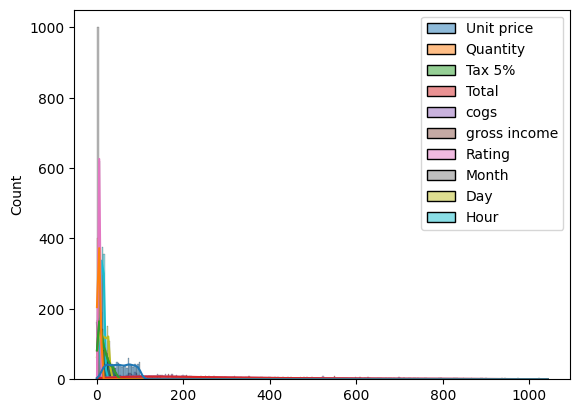
\includegraphics[width=0.5\textwidth]{Chapters/ch2/ch_2_line_graph_1.png}
    % \caption{This is an example image.}
    % \label{fig:example}
\end{figure}

Clearly, the histogram is not totally symmetric. Histograms depicting normal distribution show bell-shaped curves, and this is not bell-shaped. Hence, the data is not normally distributed.

\textbf{b) Quantile-Quantile (Q-Q) Plot} 
\newline 
\begin{figure}[h]
    \centering
    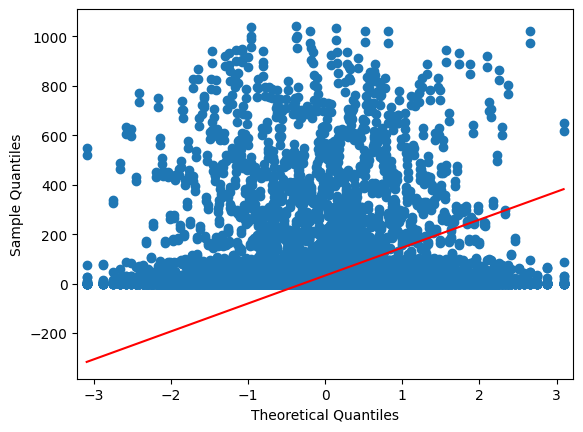
\includegraphics[width=0.5\textwidth]{Chapters/ch2/ch_2_scatter_plot_1.png}
    % \caption{This is an example image.}
    % \label{fig:example}
\end{figure}

In a Q-Q plot, if the points fall approximately along a straight line, the data is likely normally distributed. As can be seen clearly here, this is not the case. Deviations from the straight red line suggest departures from normality. 
\newline
Hence, by both the visual inspections we have inferred that the dataset is not normally distributed. 
Another way of checking for data normality is by conducting statistical tests. 

\subsubsection{Statistical Test (Shapiro-Wilk Test) }
Upon conducting this test on our dataset, I got the following output: 
\newline
Shapiro-Wilk Test: Statistic = 0.31571829319000244, p-value = 0.0
\newline
Since the p-value is lower than the chosen significance level (0.05), we can reject the null hypothesis; the data is not normally distributed.
\newline
Hence, both the visual and statistical tests have led us to believe that the data is not normally distributed and hence required normalization or standardization. But which one is suitable for our specific dataset and why?

\subsection{Which Features require Standardization and why?}
Standardization becomes essential when examining features with numeric values, especially those displaying significant scale variations. The features that benefited from standardization include:


\begin{itemize}
\item Unit price: The prices of different products can vary widely, and standardizing this feature ensures that the magnitude of the price doesn't disproportionately influence other features during model training.
\item Quantity: The number of items purchased can also exhibit considerable variability, and standardization aids in rendering this feature comparable with others.
\item Tax 5\%, Total, cogs, gross income: These features represent monetary values and may have different scales. Standardization is instrumental in ensuring that these monetary metrics are on a consistent scale, facilitating fair comparison.
\item Rating: While this feature might not necessarily demand standardization if it already falls within a specific range, if the rating scale significantly differs from other features, standardization becomes beneficial in maintaining uniformity across all features.
\end{itemize}

\subsection{Choosing between Normalization and Standardization}
\begin{itemize}
\item Magnitude Differences: Standardization is robust to features with different scales, making it suitable for datasets where features like "Unit price," "Quantity," etc., may have different magnitudes.
\item Outliers: Standardization is less sensitive to outliers compared to normalization, which can be beneficial in real-world datasets that might have some outliers.
\item Algorithms Sensitivity: Many machine learning algorithms, including those used in data mining, can benefit from standardized features, especially when they involve calculations of distances or gradients.
\end{itemize}


\subsection{Using StandardScaler}
Before applying standardization, it is important to exclude the target column. Since we want to predict target values as they are in the original dataset, we do not apply any preprocessing like encoding or standardization to the target variable. The code involved in the actual standardization is basically 2 lines:
\begin{lstlisting}[language=Python, frame=none]
scaler = StandardScaler()
df_standardized[features] = scaler.fit_transform(df_standardized[features])
\end{lstlisting}

This code creates an instance of the StandardScaler class from scikit-learn. The StandardScaler is a transformer that standardizes features by removing the mean and scaling to unit variance. 
The \verb|fit_transform| method calculates the mean and standard deviation of each selected column and then applies the standardization formula:
\begin{equation}
Standardized Value = Original Value-Mean/Standard Deviation
\end{equation}

\begin{figure}[h]
    \centering
    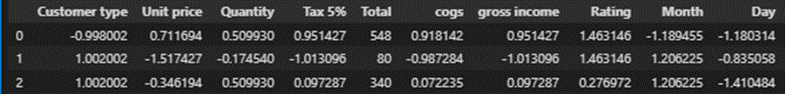
\includegraphics[width=1\textwidth]{Chapters/ch2/data_1.png}
    \caption{Sample of a few features from the standardized dataset}
    % \label{fig:example}
\end{figure}

\subsection{How did this step contribute to effective data mining?}

\begin{itemize}
\item Improved Model Convergence: Standardizing features helped machine learning models converge faster during training, especially for algorithms that relied on gradient descent optimization.
\item Enhanced Model Performance: Standardization ensured that each feature contributed equally to the model, preventing features with larger scales from dominating the learning process. This led to better model performance and generalization.
\item Facilitated Interpretation: Standardization made it easier to interpret the coefficients of the features in linear models. This was important for understanding the impact of each feature on the target variable.
\item Increased Robustness: Scaling using StandardScaler made models more robust to variations in the data and helped avoid numerical instability issues during training data and helped avoid numerical instability issues during training.
\end{itemize}

% ---------------------------------------------------------------------------------------------------

\section{Feature Selection } 
I employed PCA to conduct feature selection. Technically, PCA makes use of both feature selection and creation. It basically ‘merges’ the top ‘k’ features together, where ‘k’ is user-defined. 
The motivation for using PCA specifically was simply because we had been taught that in depth, and I wanted to try it out. Choosing ‘k’ was the main factor.



\subsection{Choosing K}
As I mentioned above, ‘k’ is the number of principal components that we are choosing to work with. Choosing this value can be a challenging task, and I utilized various means to try and understand what the ideal value could be.

\begin{figure}[h]
    \centering
    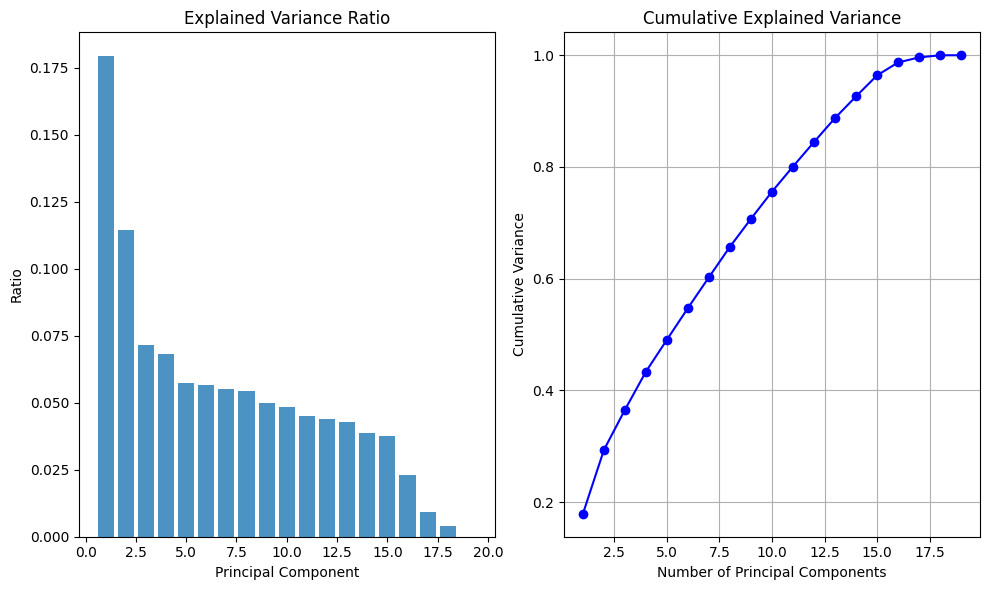
\includegraphics[width=0.7\textwidth]{Chapters/ch2/ch2_vr_er_1.png}
    % \caption{This is an example image.}
    % \label{fig:example}
\end{figure}
\begin{figure}[h]
    \centering
    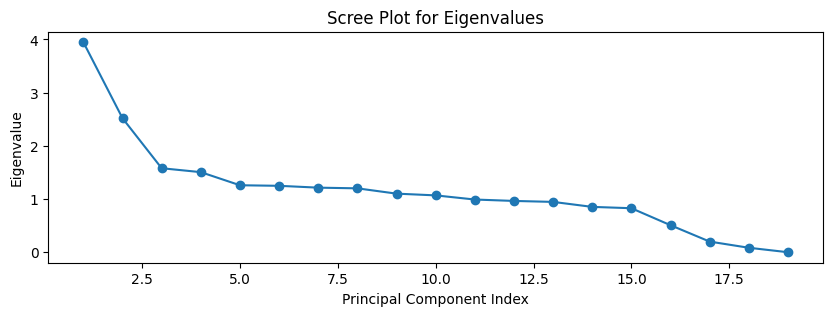
\includegraphics[width=0.7\textwidth]{Chapters/ch2/ch_2_screeplot_1.png}
    % \caption{This is an example image.}
    % \label{fig:example}
\end{figure}
\newpage
After analyzing these charts, I decided to initially start by experimenting with ‘k’ at 15. The most efficient way of finding the ideal value for ‘k’ is by trial and error. But using these means can help figure out a good starting point.
% -----------------------------------------------------------------------------------------------------


\section{Splitting Data}

\subsection{Importance of splitting}

\begin{itemize}
\item Avoids Overfitting: Imagine training your model on the same data you use to evaluate it. It would be like memorizing the answers in a test instead of truly understanding the concepts. The model might perform well on that specific data (high training accuracy), but it wouldn't generalize well to new, unseen data (low testing accuracy). Splitting the data prevents this "memorization" by reserving the testing set for unbiased evaluation.
\item Provides Unbiased Evaluation: Training the model only on the training set eliminates any influence from the testing data. This ensures the evaluation metrics (e.g., R-squared, mean squared error) reflect the model's true performance on unseen data, making it a reliable measure of its generalizability.
\item Helps Tune Hyperparameters: Hyperparameters are knobs that influence the model's learning process. Splitting the data allows you to experiment with different hyperparameter values on the training set, evaluating their impact on performance through the validation set, and finally selecting the best performing configuration for the final model.
\item Identifies Data Leakage: Data leakage occurs when information from the testing set somehow influences the training process. For example, including future values in a time series prediction might give the model an unfair advantage in training. Splitting the data minimizes this risk and leads to a more accurate assessment of the model's true capabilities.
\item Facilitates Cross-Validation: Splitting the data can be extended to cross-validation techniques, where the dataset is further divided into multiple folds. Each fold is used for training and testing in turn, providing a more robust and statistically sound evaluation of the model's performance across different data subsets.
\end{itemize}
% =================================================
\subsection{Applying Train-Test Split}

The \verb|train_test_split| function from the \verb|scikit-learn| library is used to split the data into training and testing sets. The parameters are as follows:
\begin{itemize}

\item X: The feature matrix (The preprocessed DataFrame)
\item y: The target variable (‘Total’)
\item \verb|test_size|: The proportion of the dataset to include in the test split. In this case, it's set to 0.2, meaning 20\% of the data will be used for testing.
\item \verb|random_state|: This is used to ensure reproducibility. Setting a seed (here, 42) means that if you run the code multiple times, you'll get the same train-test split each time.

\end{itemize}

The resulting dimensions of both sets:
\verb|X_train shape: (800, 22)|,
\verb|X_test shape: (200, 22)|,
\verb|y_train shape: (800,)|,
\verb|y_test shape: (200,)|


% --------------------------------------------------------------------------------------------------------

